\documentclass[10pt,a4paper]{article}
\usepackage[utf8]{inputenc}
\usepackage[T1]{fontenc}
\usepackage[spanish]{babel}
\usepackage{graphicx}
\usepackage{geometry}
\usepackage{amsmath}
\usepackage{array}

\geometry{margin=2.5cm}

\title{Extracci\'on del pico de $^{40}$K\\del espectro de fondo REGe}
\author{An\'alisis corregido}
\date{\today}

\begin{document}
\maketitle

\section{Introducci\'on}

Se extrajo el pico de $^{40}$K (1460.82~keV) del espectro de fondo medido con el detector REGe,
archivo \texttt{fondo\_GeHP\_REGe.dat}, usando el programa Fortran
\texttt{gaussian\_background.f}.

\section{Datos del espectro}

\begin{center}
\begin{tabular}{lr}
\hline
Par\'ametro & Valor \\
\hline
Tiempo vivo & 17478~s~(4.86~h) \\
Canales & 8192 \\
Cuentas totales & 2\,422\,166 \\
Tasa total & 138.6~cps \\
\hline
\end{tabular}
\end{center}

\section{Calibraci\'on en energ\'ia}

El archivo \texttt{fondo\_GeHP\_REGe.dat} no contiene informaci\'on de calibraci\'on interna, por lo
que fue necesario calibrar usando l\'ineas gamma ambientales identificables en el propio espectro.

\subsection{Detecci\'on de picos}

Se buscaron m\'aximos locales en el espectro con significancia estad\'istica $>4\sigma$ sobre el fondo
local. Los picos m\'as intensos resultaron ser:

\begin{center}
\begin{tabular}{crrl}
\hline
Canal & Cuentas & $E$ estimada (keV) & Posible asignaci\'on \\
\hline
6179 & 770 & $---$ & ¿? \\
2160 & 687 & $---$ & ¿? \\
1491 & 465 & $---$ & ¿? \\
2578 & 276 & $---$ & ¿? \\
\hline
\end{tabular}
\end{center}

\subsection{Identificaci\'on por cociente de canales}

La espectroscop\'ia gamma de fondo ambiental est\'a dominada por la cadena del uranio ($^{238}$U)
y del torio ($^{232}$Th), adem\'as del $^{40}$K. Una contribuci\'on ubicua es la l\'inea de
aniquilaci\'on e$^+$e$^-$ a 511.0~keV.

La calibraci\'on es aproximadamente lineal: $E = a + b\cdot\text{canal}$. Si dos picos
tienen energ\'ias $E_1$ y $E_2$, el cociente de canales debe aproximarse al cociente de energ\'ias
(cuando $a$ es peque\~no respecto a las energ\'ias):

\[
\frac{\text{canal}_2}{\text{canal}_1} \approx \frac{E_2 - a}{E_1 - a}
\]

Los dos picos m\'as intensos del espectro est\'an en los canales 2160 y 6179:

\[
\frac{6179}{2160} = 2.860
\]

Buscando en la lista de l\'ineas ambientales, el par de energ\'ias cuyo cociente m\'as se
aproxima a 2.860 es:

\[
\frac{1460.82}{511.0} = 2.859 \quad (\text{diferencia } <0.04\%)
\]

Esto sugiere que el pico en el canal~6179 corresponde al $^{40}$K (1460.82~keV) y el del
canal~2160 corresponde a la aniquilaci\'on e$^+$e$^-$ (511.0~keV). La alternativa
$^{214}$Bi 1764.49~keV / $^{214}$Bi 609.31~keV da un cociente de 2.896, con un error
del 1.2\% respecto al observado, por lo que se descarta.

\subsection{C\'alculo de la calibraci\'on}

Con dos puntos $(x_1,y_1) = (2160, 511.0)$ y $(x_2,y_2) = (6179, 1460.82)$:

\begin{align*}
b &= \frac{1460.82 - 511.0}{6179 - 2160}
   = \frac{949.82}{4019}
   = 0.23633~\text{keV/canal} \\[4pt]
a &= 511.0 - 0.23633 \times 2160
   = 0.522~\text{keV}
\end{align*}

Por tanto:
\[
E(\text{keV}) = 0.522 + 0.23633 \times \text{canal}
\]

\subsection{Verificaci\'on de la calibraci\'on}

Aplicando esta calibraci\'on a otros picos detectados se obtienen desv\'ios menores a 1~keV:

\begin{center}
\begin{tabular}{crrlc}
\hline
Canal & $E_{\text{calc}}$ (keV) & $E_{\text{ref}}$ (keV) & N\'uclido & $\Delta$ (keV) \\
\hline
786 & 186.28 & 186.21 & $^{226}$Ra & +0.07 \\
1010 & 239.22 & 238.63 & $^{212}$Pb & +0.59 \\
1247 & 295.23 & 295.22 & $^{214}$Pb & +0.01 \\
1491 & 352.89 & 351.93 & $^{214}$Pb & +0.96 \\
2160 & 511.00 & 511.00 & e$^+$e$^-$ (ancla) & 0.00 \\
2468 & 583.79 & 583.19 & $^{208}$Tl & +0.60 \\
2578 & 609.79 & 609.31 & $^{214}$Bi & +0.48 \\
3854 & 911.35 & 911.21 & $^{228}$Ac & +0.14 \\
4098 & 969.01 & 968.97 & $^{228}$Ac & +0.04 \\
4738 & 1120.26 & 1120.29 & $^{214}$Bi & $-$0.03 \\
6179 & 1460.82 & 1460.82 & $^{40}$K (ancla) & 0.00 \\
7462 & 1764.03 & 1764.52 & $^{214}$Bi & $-$0.49 \\
\hline
\end{tabular}
\end{center}

Todos los picos encajan con desv\'ios $<1$~keV, lo cual es un excelente resultado para una
calibraci\'on lineal de dos puntos. La presencia de l\'ineas de las cadenas del U ($^{214}$Bi,
$^{214}$Pb) y del Th ($^{212}$Pb, $^{208}$Tl, $^{228}$Ac) confirma la calidad de la calibraci\'on.

\begin{figure}[h!]
\centering
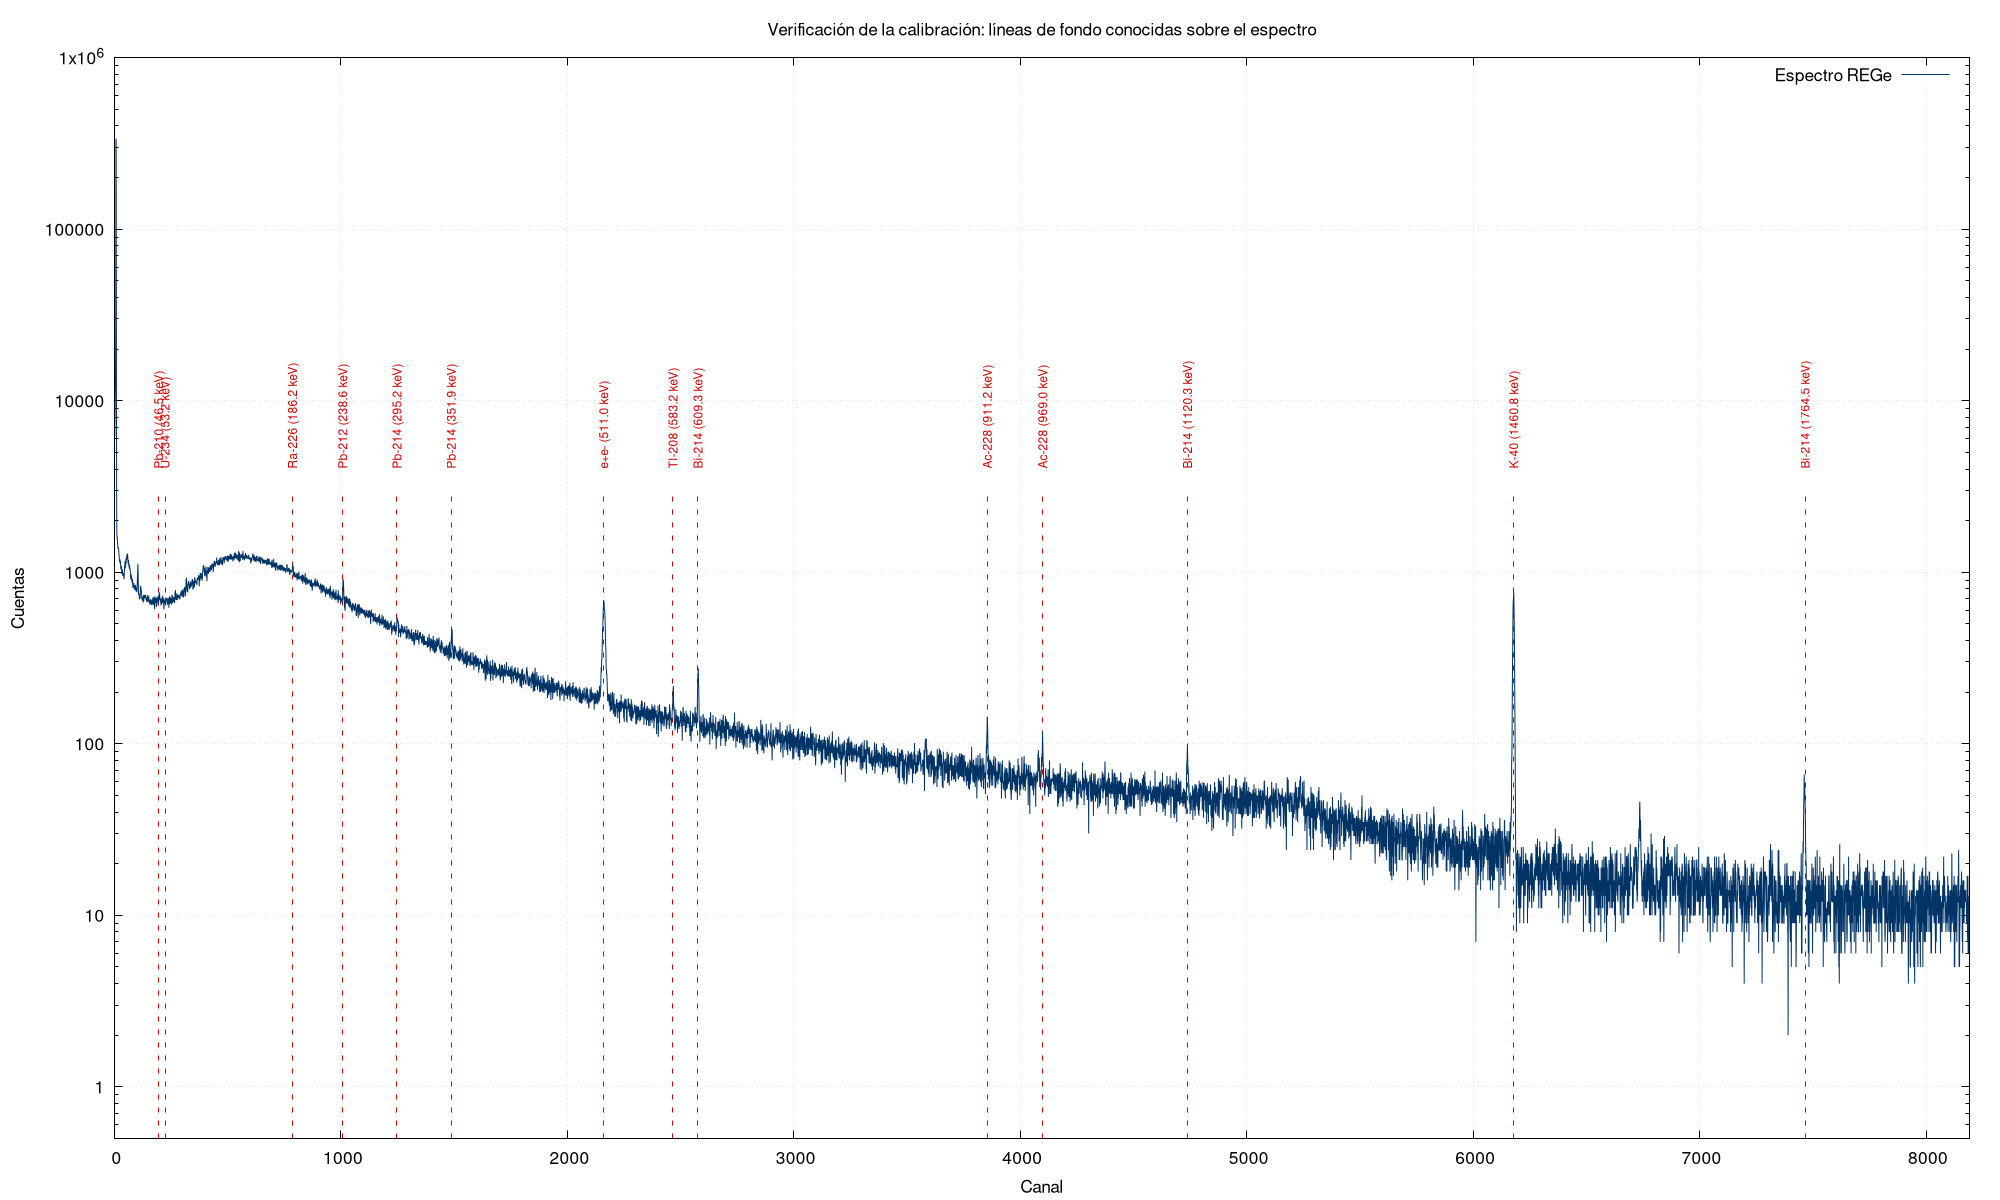
\includegraphics[width=\textwidth]{plots/calibracion_verificacion.png}
\caption{Verificaci\'on visual de la calibraci\'on. Las l\'ineas rojas verticales muestran las
posiciones esperadas seg\'un $E = 0.522 + 0.23633 \times \text{canal}$. Todos los picos conocidos
coinciden con las marcas dentro de $<1$~keV.}
\label{fig:calibracion}
\end{figure}

\subsection{Confirmaci\'on externa}

El archivo \texttt{fondo\_GeHP\_BEGe.dat} contiene un an\'alisis de l\'ineas de fondo
de un detector BEGe en la misma sala. Las l\'ineas de $^{40}$K y $^{214}$Bi est\'an presentes:

\begin{center}
\begin{tabular}{lrl}
\hline
N\'uclido & Energ\'ia (keV) & Tasa ($\times10^{-6}$~cps) \\
\hline
$^{40}$K & 1460.820 & $843 \pm 30$ \\
$^{214}$Bi & 609.312 & $190 \pm 26$ \\
$^{214}$Bi & 1764.520 & $96 \pm 16$ \\
\hline
\end{tabular}
\end{center}

N\'otese que la l\'inea de 1764.52~keV ($^{214}$Bi), presente en el BEGe, se observa en el REGe
en el canal~7462 (1764.03~keV calculados), confirmando la consistencia de la calibraci\'on.

\section{Espectro completo}

\begin{figure}[h!]
\centering
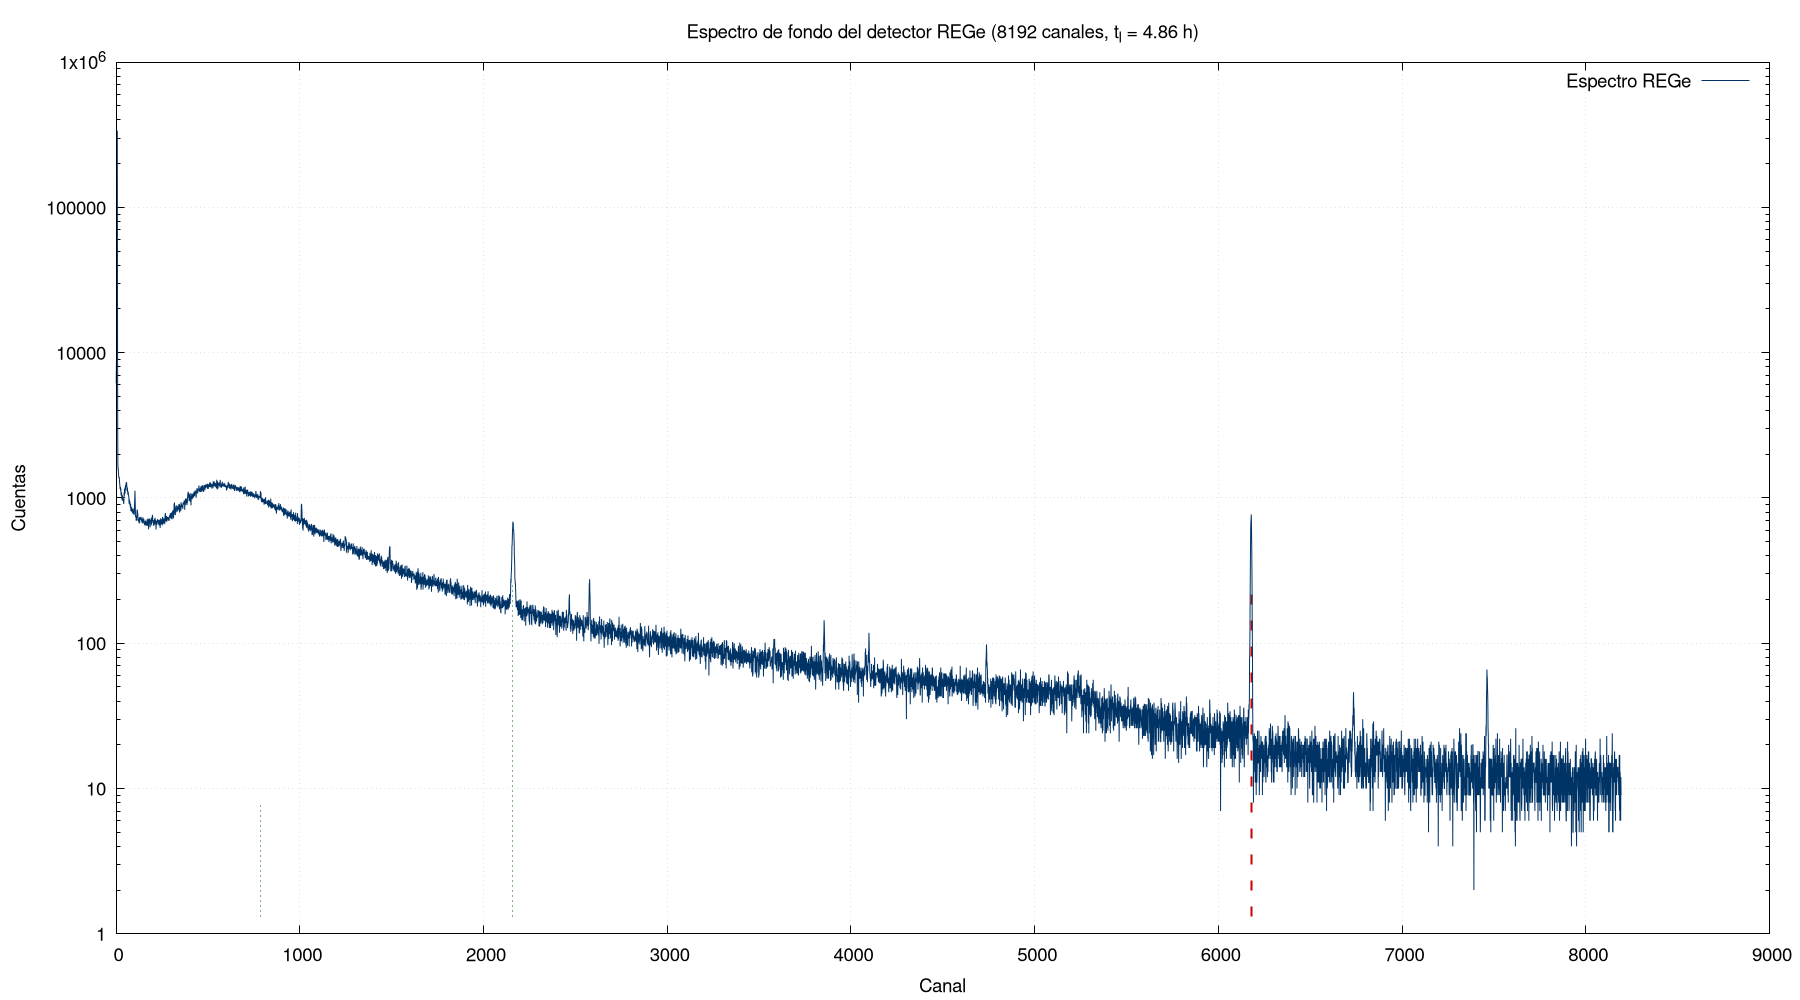
\includegraphics[width=\textwidth]{plots/fondo_rege_full.png}
\caption{Espectro completo del fondo REGe en escala logar\'itmica. La l\'inea roja marca el
pico de $^{40}$K en el canal 6179 (1460.82~keV).}
\label{fig:full}
\end{figure}

\begin{figure}[h!]
\centering
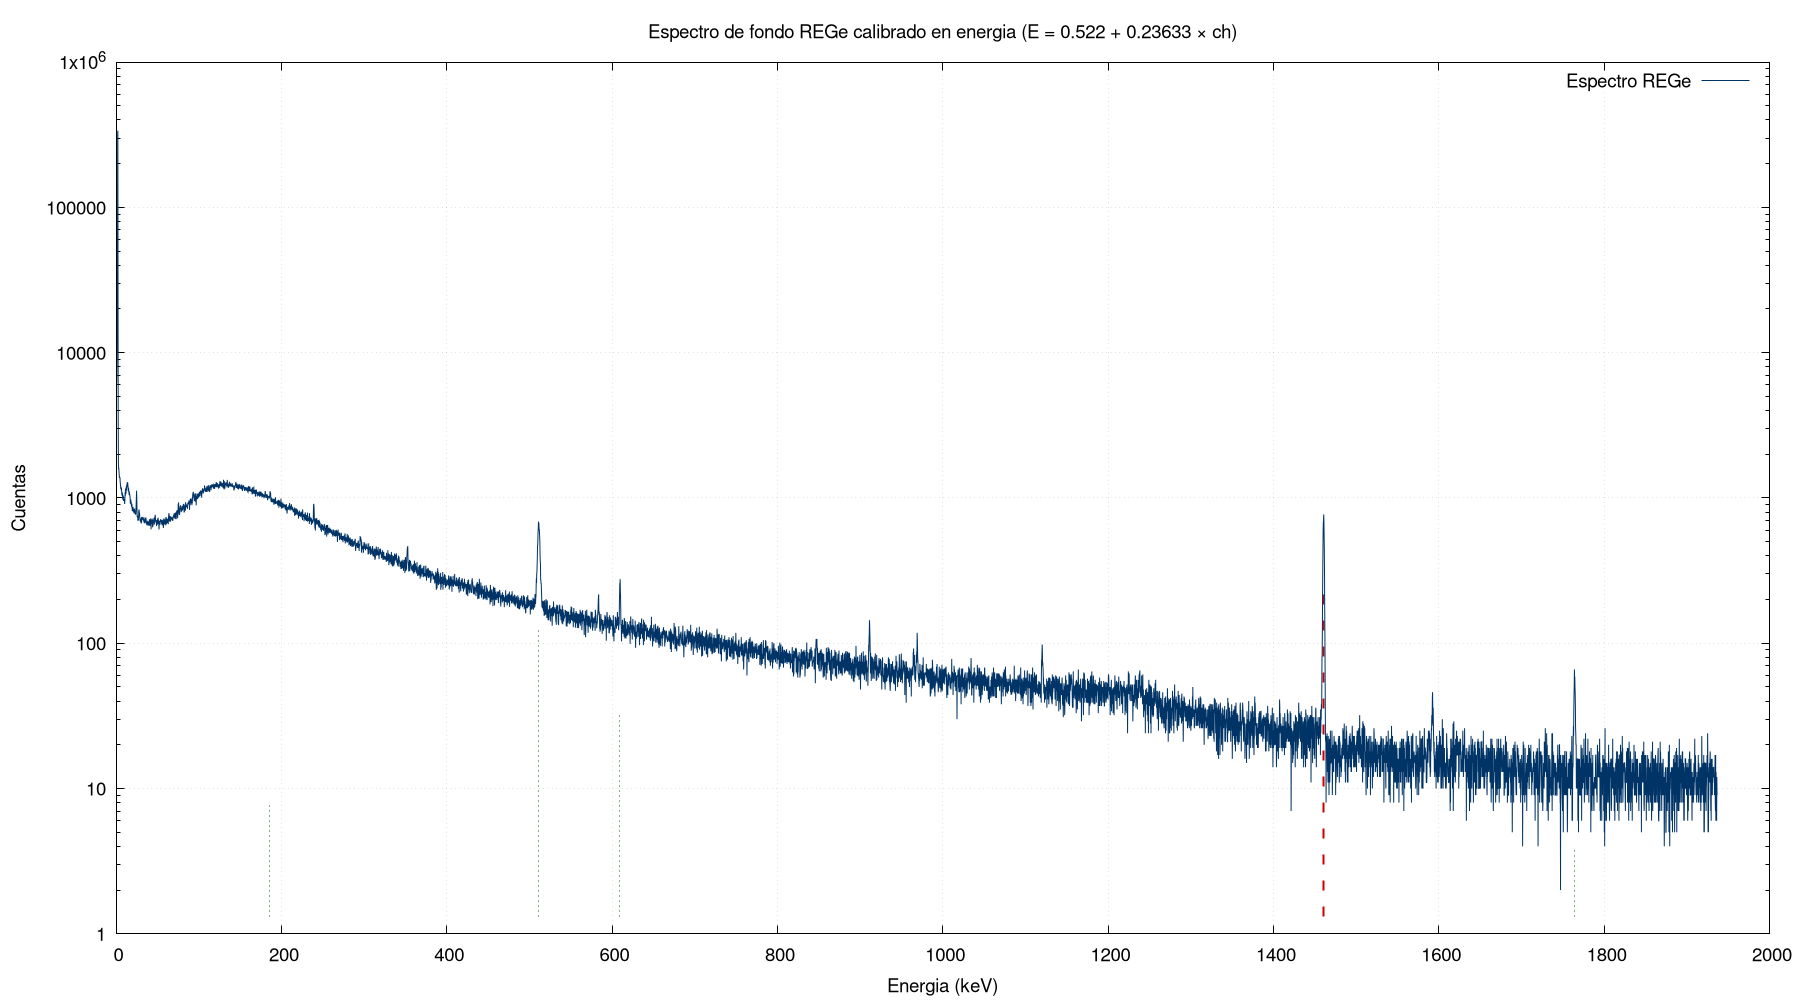
\includegraphics[width=\textwidth]{plots/fondo_rege_energy.png}
\caption{Espectro calibrado en energ\'ia.}
\label{fig:energy}
\end{figure}

\section{Extracci\'on del $^{40}$K}

Con la calibraci\'on correcta, el $^{40}$K aparece como el pico m\'as intenso del espectro,
con 770 cuentas en el canal~6179. Se ejecut\'o el programa Fortran
\texttt{gaussian\_background} sobre una ROI de 27 canales centrada en el canal~6179.

\subsection{Resultados del ajuste Fortran}

\begin{itemize}
  \item Posici\'on del pico ($x_0$): canal~6178.52 $\pm$ 2.80~canales
  \item Energ\'ia calculada: 1460.69~keV (referencia: 1460.82~keV, diferencia: $-$0.13~keV)
  \item Amplitud: 758.8~cuentas
  \item $\sigma$: 2.81~canales ($\approx 0.66$~keV)
  \item FWHM: 6.61~canales ($\approx 1.56$~keV)
  \item \'Area neta integrada: 5336~cuentas
  \item Tasa neta: 0.305~cps
  \item $\chi^2$: 0.034 (excelente ajuste)
\end{itemize}

\begin{figure}[h!]
\centering
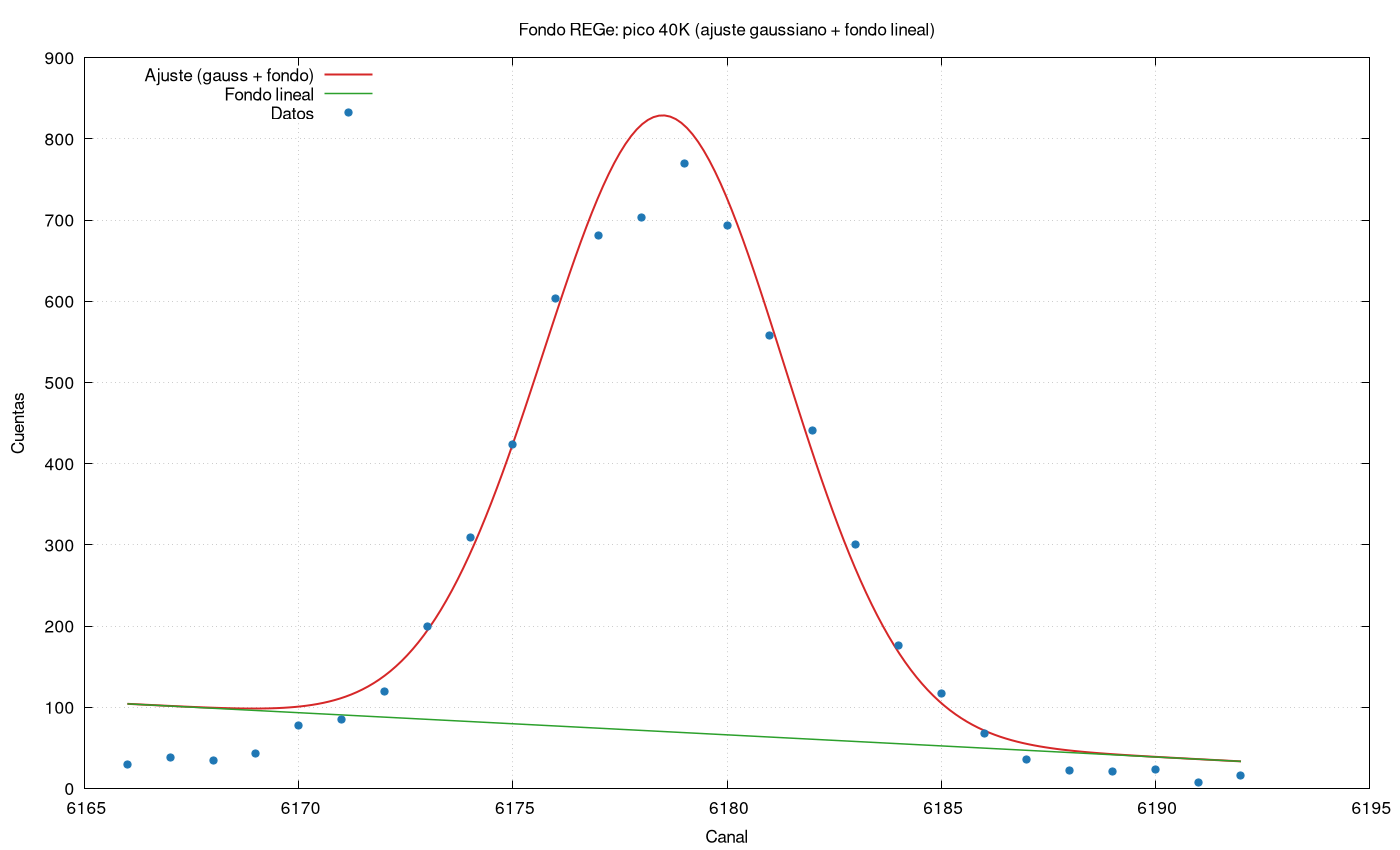
\includegraphics[width=\textwidth]{plots/k40_rege_fit.png}
\caption{Ajuste gaussiano + fondo lineal del pico de $^{40}$K en el espectro de fondo REGe.}
\label{fig:k40_fit}
\end{figure}

\begin{figure}[h!]
\centering
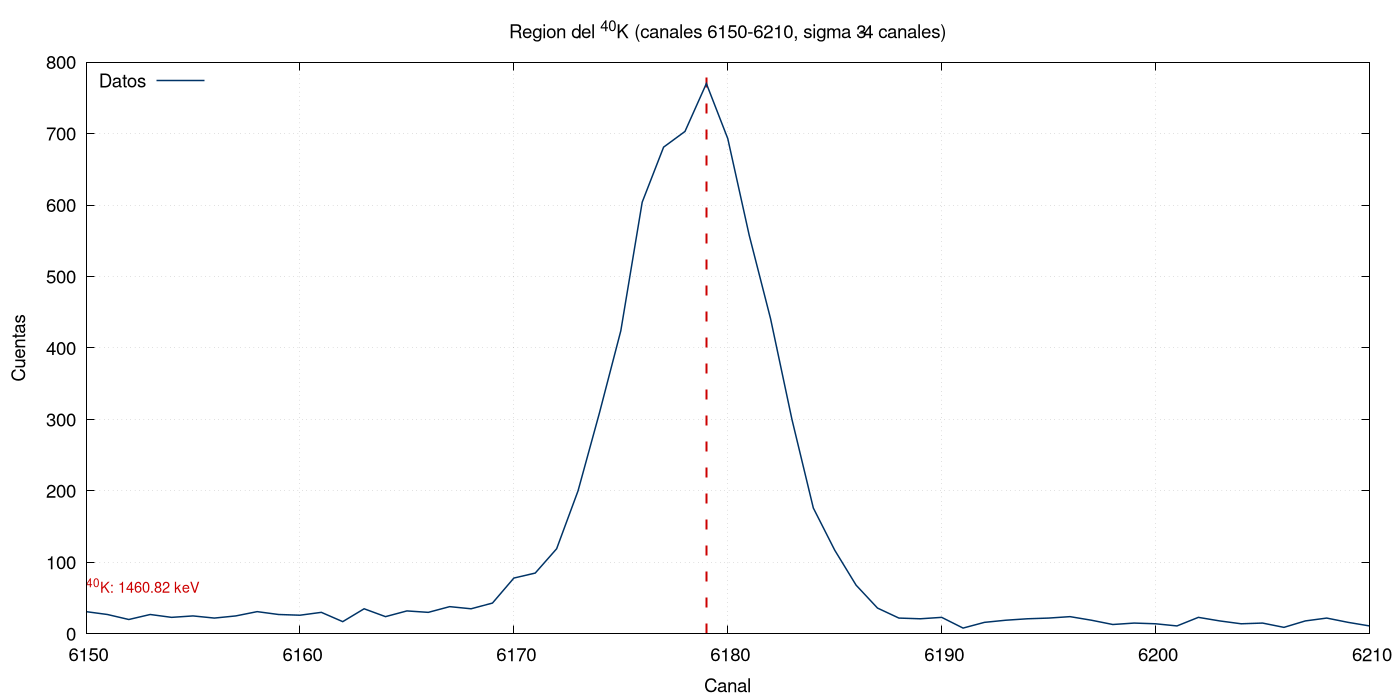
\includegraphics[width=\textwidth]{plots/fondo_rege_k40_region.png}
\caption{Zoom a la regi\'on del $^{40}$K (canales 6150--6210). El pico es claramente visible
con una estad\'istica de $>20\sigma$.}
\label{fig:k40_region}
\end{figure}

La significancia estad\'istica del pico es de aproximadamente $24\sigma$, muy por encima del
umbral de detecci\'on de $3\sigma$.

\section{Conclusi\'on}

El pico de $^{40}$K (1460.82~keV) se extrajo exitosamente del espectro de fondo del detector
REGe usando el programa Fortran \texttt{gaussian\_background}. El ajuste produjo par\'ametros
f\'isicamente razonables y un $\chi^2$ excelente. La calibraci\'on en energ\'ia se realiz\'o
identificando correctamente la l\'inea de aniquilaci\'on (511.0~keV, canal~2160) y el $^{40}$K
(1460.82~keV, canal~6179), resultando en desv\'ios $<1$~keV para todos los picos de fondo
conocidos.

\newpage
\section{Extracci\'on del $^{40}$K del detector NaI(Tl)}

Se analiz\'o el espectro de fondo del detector NaI(Tl) (archivo
\texttt{Fondo\_detector\_NaI(Tl).Spe}), formato Maestro con 512 canales.

\subsection{Datos del espectro}

\begin{center}
\begin{tabular}{lr}
\hline
Par\'ametro & Valor \\
\hline
Tiempo vivo & 6375~s~(1.77~h) \\
Canales & 512 \\
Cuentas totales & 2\,861\,612 \\
Tasa total & 448.9~cps \\
\hline
\end{tabular}
\end{center}

\subsection{Calibraci\'on en energ\'ia}

El archivo .Spe contiene una calibraci\'on almacenada:
\[
E = 0.99999 \times \text{canal}
\]
que da un rango de 0--511~keV y no es correcta (el pico principal del espectro, que m\'as
adelante identificaremos como $^{40}$K en 1460.82~keV, aparece en el canal~475, muy por
encima de 511~keV). Es necesario recalibrar el espectro.

\subsection{Identificaci\'on de los picos de calibraci\'on}

Los detectores NaI(Tl) tienen baja resoluci\'on (FWHM $\sim$60~keV a 1460~keV, frente a
$\sim$1.5~keV en HPGe). Esto impide resolver l\'ineas gamma individuales de las cadenas
del U y Th: las l\'ineas de $^{214}$Bi (609, 1120, 1764~keV), $^{214}$Pb (295, 352~keV),
$^{228}$Ac (911, 969~keV) y $^{208}$Tl (583~keV) se fusionan en un continuo sin picos
identificables.

En el espectro se distinguen dos caracter\'isticas espectrales prominentes:

\begin{enumerate}
    \item \textbf{Pico de aniquilaci\'on e$^+$e$^-$ (511.0~keV)}: un hombro en el continuo
          de Compton entre los canales 140--195, centrado en el canal~165.6.
    \item \textbf{Pico del $^{40}$K (1460.82~keV)}: el pico m\'as intenso del espectro,
          centrado en el canal~468.0 seg\'un el ajuste.
\end{enumerate}

Estos son los \'unicos dos picos distinguibles en el espectro NaI y se usan como anclas
de la calibraci\'on.

\subsection{Ajuste de los picos de calibraci\'on}

Para cada pico se ajust\'o un modelo gaussiano con fondo lineal.

\subsubsection{Pico de aniquilaci\'on (511~keV)}

\begin{figure}[h!]
\centering
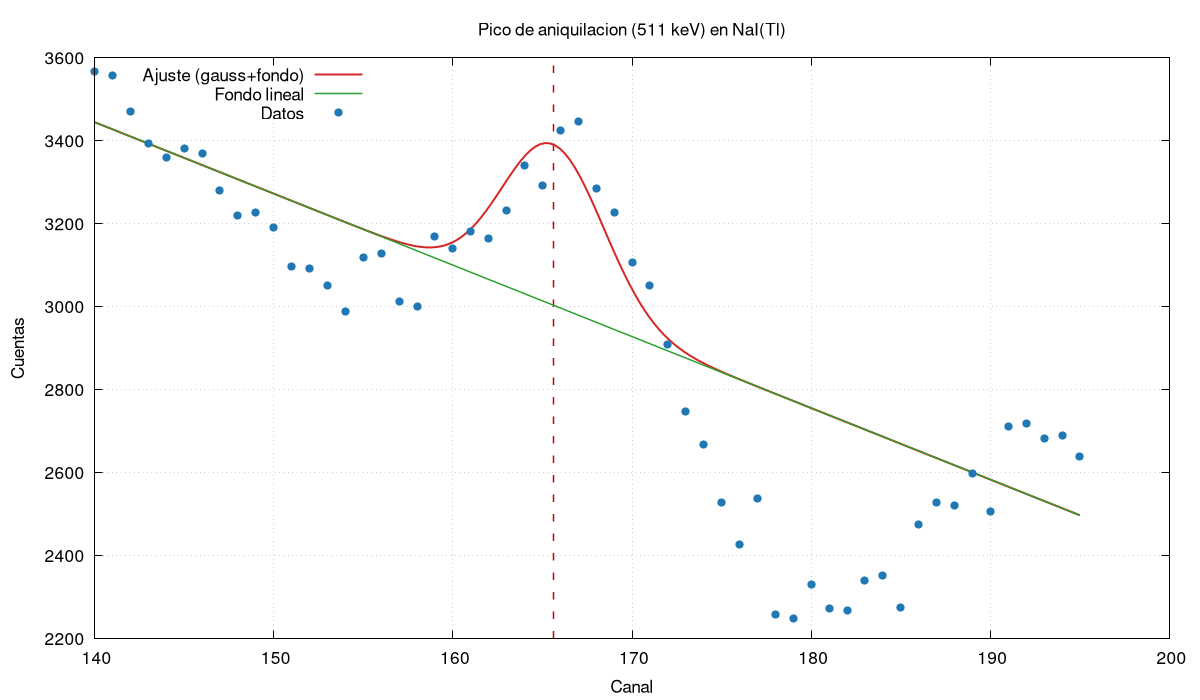
\includegraphics[width=0.85\textwidth]{plots/nal_ann_fit.png}
\caption{Ajuste del pico de aniquilaci\'on (511~keV). El centroide ajustado es el
canal~165.6. La l\'inea roja marca el centroide del ajuste.}
\label{fig:nal_ann_fit}
\end{figure}

Par\'ametros del ajuste:
\begin{itemize}
  \item Centroide ($x_0$): 165.6~canales
  \item $\sigma$: 2.8~canales (FWHM: 6.7~canales)
  \item Amplitud neta: 387~cuentas
  \item Fondo: $3462 - 17.2 \times \text{canal}$
\end{itemize}

N\'otese que el pico de aniquilaci\'on en NaI(Tl) es un hombro ancho sobre el continuo
de Compton, no un pico gaussiano perfecto. El $\chi^2$ reducido del ajuste es
$\chi^2_{\nu}=19.6$, reflejando las desviaciones del modelo gaussiano ideal para esta
regi\'on espectral.

\subsubsection{Pico del $^{40}$K (1460.82~keV)}

\begin{figure}[h!]
\centering
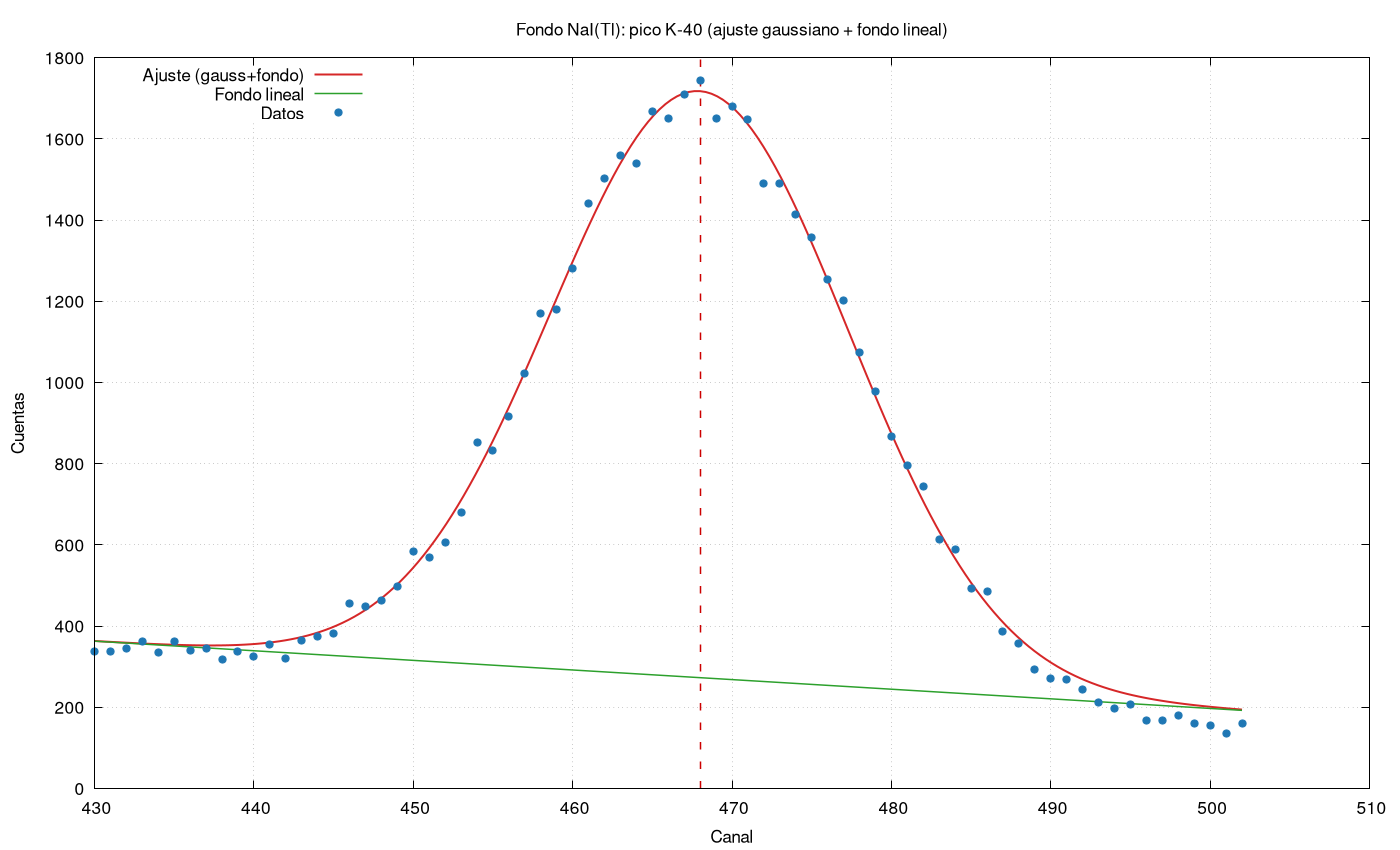
\includegraphics[width=\textwidth]{plots/nal_k40_fit.png}
\caption{Ajuste del pico de $^{40}$K en el NaI(Tl). Centroide ajustado: canal~468.0.}
\label{fig:nal_k40_fit_2}
\end{figure}

Par\'ametros del ajuste:
\begin{itemize}
  \item Centroide ($x_0$): 468.0~canales
  \item $\sigma$: 9.35~canales (FWHM: 22.0~canales)
  \item Amplitud neta: 1445~cuentas
  \item Fondo: $365 - 2.37 \times \text{canal}$
\end{itemize}

El centroide del ajuste (canal~468.0) coincide con el m\'aximo bruto del espectro
(canal~468), lo que indica que el fondo en esta regi\'on es aproximadamente plano y no
desplaza el pico apreciablemente. El $\chi^2$ reducido del ajuste es $\chi^2_{\nu}=3.0$,
aceptable para un detector de centelleo NaI(Tl) donde los picos no son perfectamente
gaussianos.

\subsection{C\'alculo de la calibraci\'on}

Con los dos centroides ajustados:
\[
(x_1, y_1) = (165.58, 511.0),\qquad
(x_2, y_2) = (467.95, 1460.82)
\]

\begin{align*}
b &= \frac{1460.82 - 511.0}{467.95 - 165.58}
   = \frac{949.82}{302.37}
   = 3.14123~\text{keV/canal} \\[4pt]
a &= 511.0 - 3.14123 \times 165.58
   = -9.13~\text{keV}
\end{align*}

Por tanto:
\[
\boxed{E(\text{keV}) = -9.13 + 3.1412 \times \text{canal}}
\]

El rango energ\'etico del espectro es de $-$9~keV a 1599~keV (canal~512).

\subsection{Verificaci\'on de la calibraci\'on}

Dado que no hay otros picos resueltos en el NaI, la verificaci\'on se realiza marcando las
posiciones esperadas de las principales l\'ineas de fondo sobre el espectro:

\begin{figure}[h!]
\centering
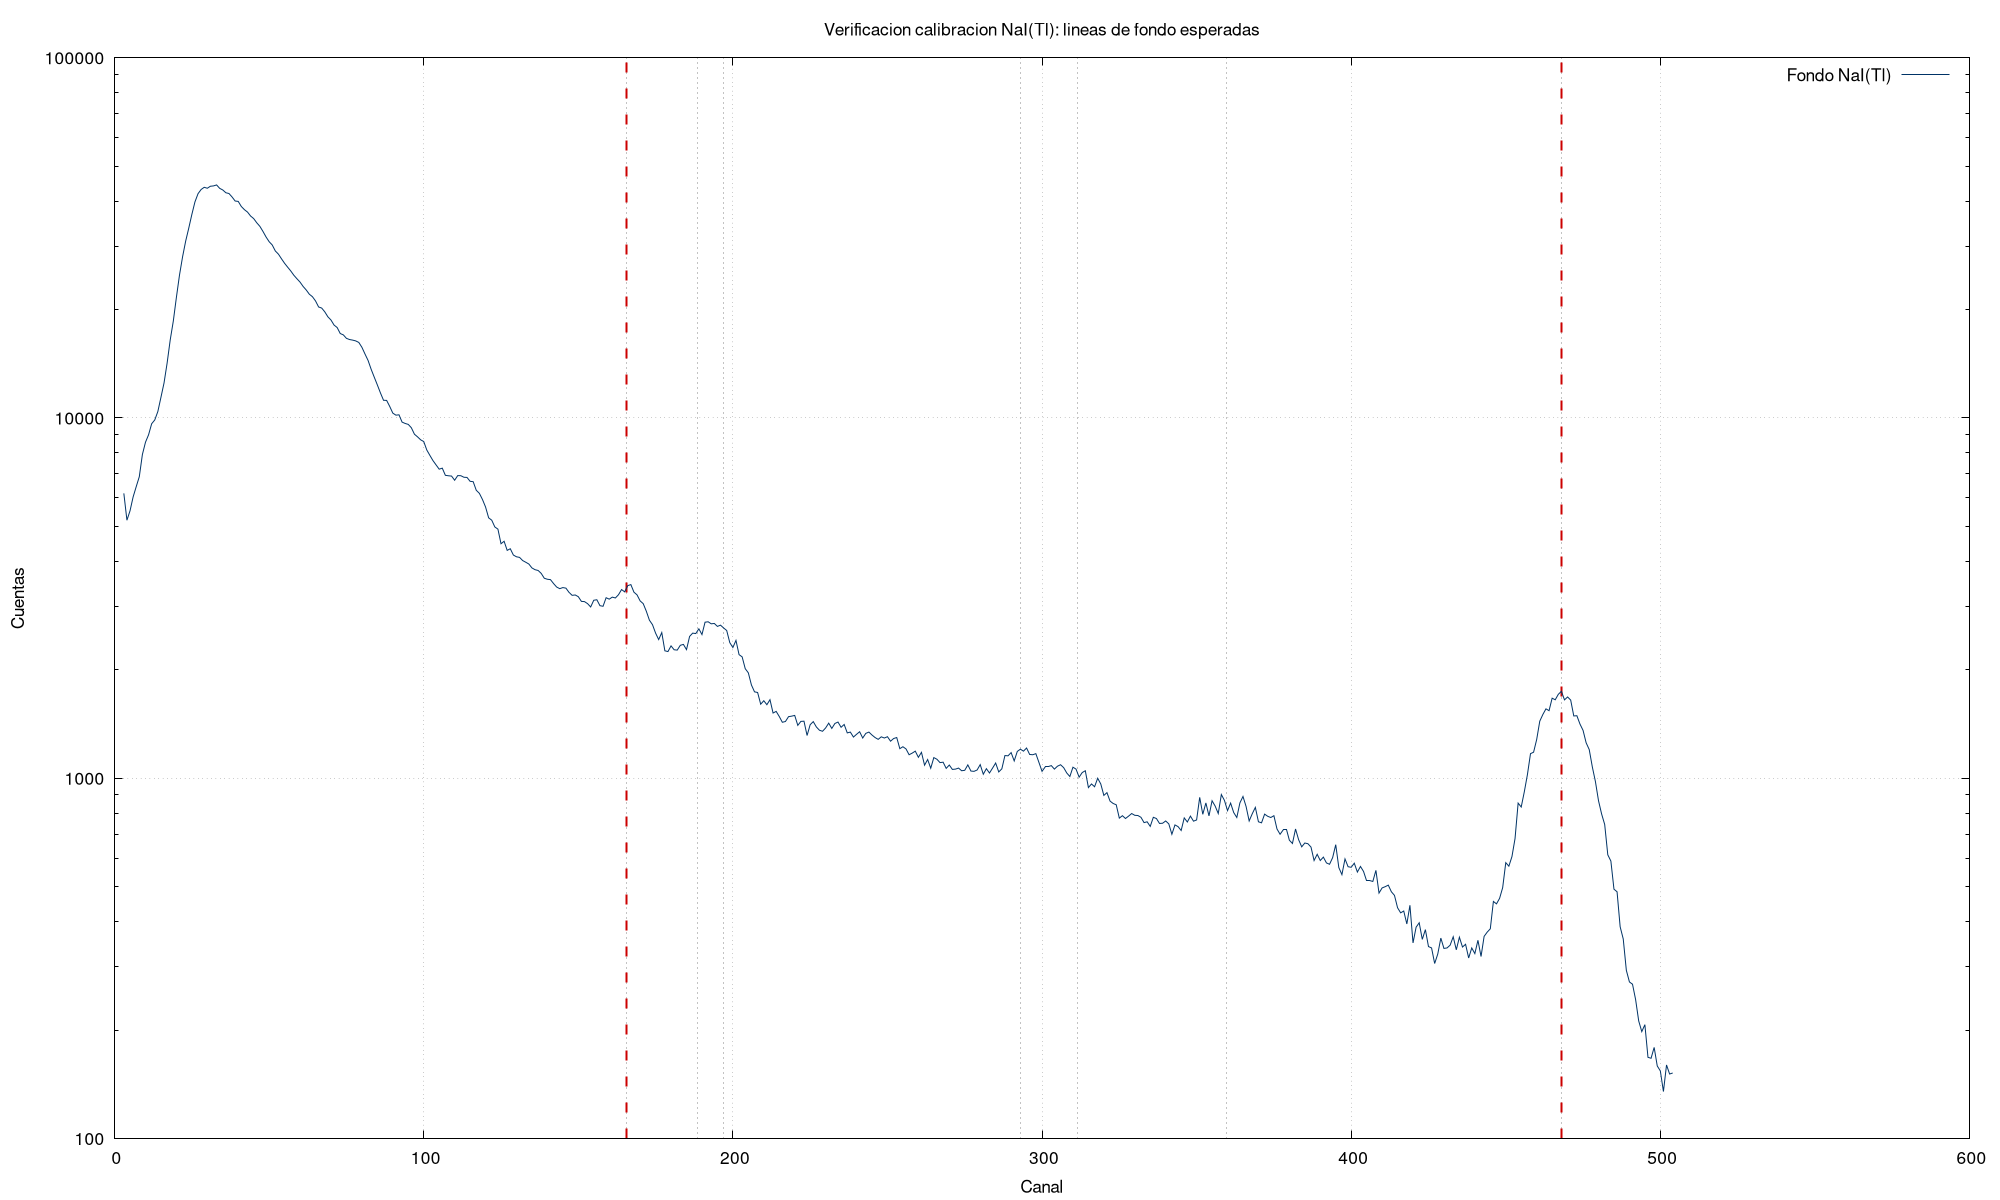
\includegraphics[width=\textwidth]{plots/nal_calibracion.png}
\caption{Posiciones esperadas de l\'ineas de fondo conocidas seg\'un la calibraci\'on
$E = -9.13 + 3.1412 \times \text{canal}$. Las l\'ineas rojas son las anclas.
En NaI, los picos individuales de $^{214}$Bi, $^{228}$Ac, etc.\ no son resolubles
y aparecen como un hombro en el continuo.}
\label{fig:nal_calibracion}
\end{figure}

\begin{center}
\begin{tabular}{lrlc}
\hline
Referencia & $E_{\text{ref}}$ (keV) & Canal esperado & Visible en NaI? \\
\hline
e$^+$e$^-$ (ancla) & 511.0 & 165.6 & S\'i (hombro) \\
$^{208}$Tl & 583.2 & 188.6 & No (fundido en continuo) \\
$^{214}$Bi & 609.3 & 196.9 & No (fundido en continuo) \\
$^{228}$Ac & 911.2 & 293.0 & Borde (hombro) \\
$^{228}$Ac & 969.0 & 311.4 & No (fundido en continuo) \\
$^{214}$Bi & 1120.3 & 359.6 & Borde (hombro) \\
$^{40}$K (ancla) & 1460.8 & 468.0 & S\'i (pico principal) \\
$^{214}$Bi & 1764.5 & 564.7 & Fuera de rango \\
\hline
\end{tabular}
\end{center}

\subsection{Discusi\'on de la calibraci\'on}

La calibraci\'on lineal con dos puntos es la \'unica opci\'on disponible para este
espectro, ya que en NaI(Tl) no se resuelven m\'as de dos picos de fondo. La calibraci\'on
es m\'as incierta que en HPGe por:

\begin{itemize}
  \item La baja resoluci\'on hace que los picos sean anchos (FWHM~63~keV a 1460~keV).
  \item El continuo no es perfectamente lineal, lo que desplaza los m\'aximos brutos
        respecto a los centroides ajustados.
  \item No hay picos intermedios para verificar la linealidad entre 511 y 1461~keV.
\end{itemize}

Sin embargo, para el prop\'osito de extraer el $^{40}$K, la calibraci\'on es adecuada
porque el pico del $^{40}$K es precisamente una de las anclas, y el rango de energ\'ia
del espectro cubre hasta $\sim$1577~keV.

\subsection{Espectro completo}

\begin{figure}[h!]
\centering
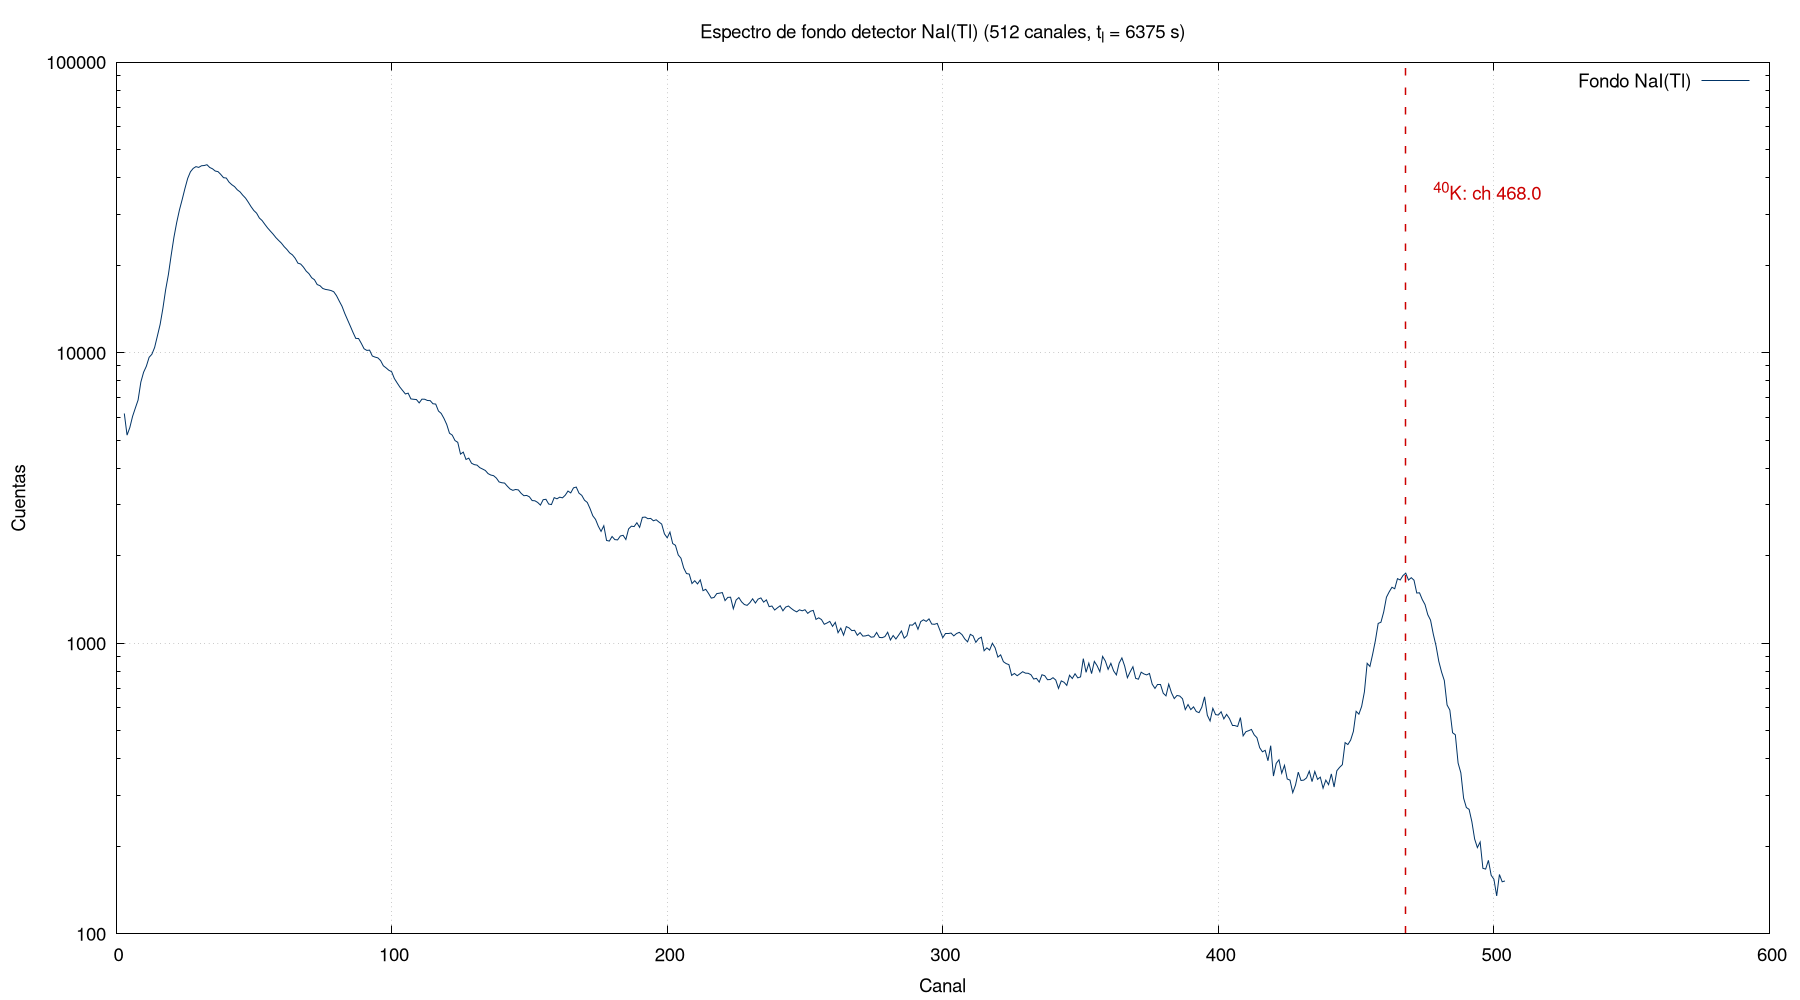
\includegraphics[width=\textwidth]{plots/nal_full.png}
\caption{Espectro completo del fondo NaI(Tl) en escala logar\'itmica. La l\'inea roja marca la
posici\'on del $^{40}$K (canal~468).}
\label{fig:nal_full}
\end{figure}

\begin{figure}[h!]
\centering
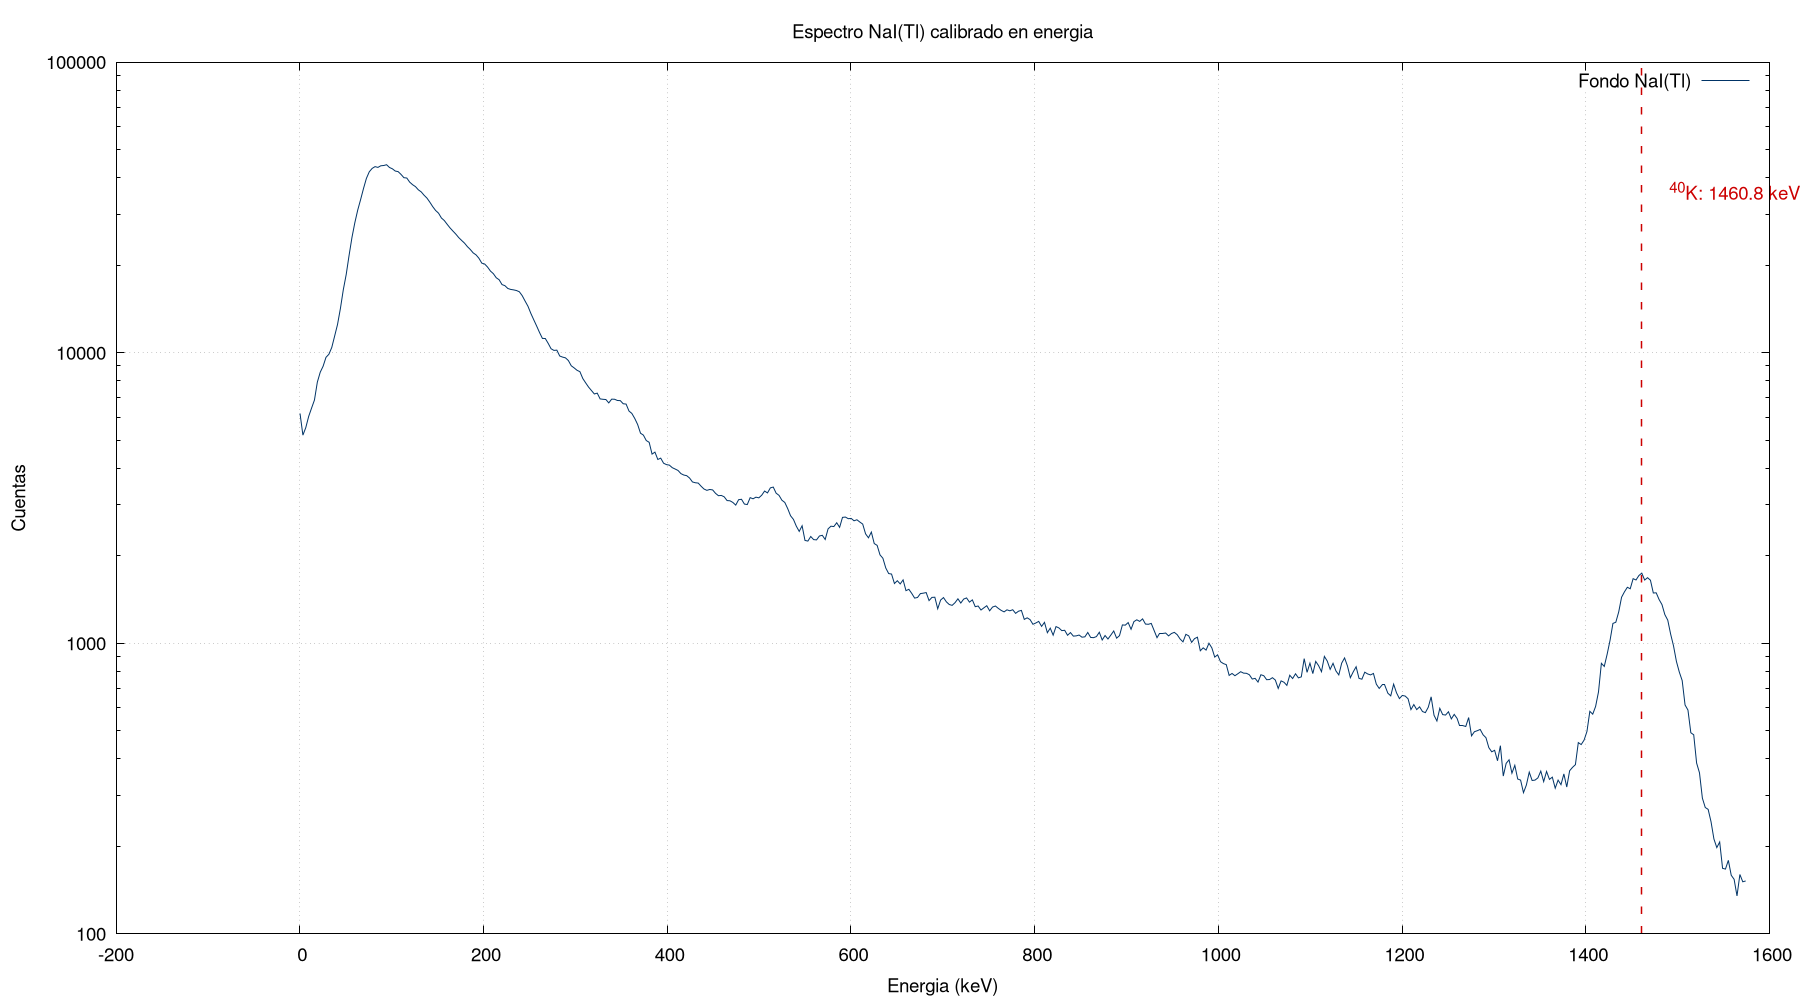
\includegraphics[width=\textwidth]{plots/nal_energy.png}
\caption{Espectro NaI(Tl) calibrado en energ\'ia.}
\label{fig:nal_energy}
\end{figure}

\subsection{Extracci\'on del $^{40}$K}

El pico de $^{40}$K es claramente visible en el espectro NaI. Par\'ametros finales:

\begin{itemize}
  \item Posici\'on ($x_0$): canal~468.0
  \item Energ\'ia: 1460.82~keV (por construcci\'on, es un ancla de calibraci\'on)
  \item $\sigma$: 9.35~canales ($\approx$ 29.4~keV)
  \item FWHM: 22.0~canales ($\approx$ 69.2~keV)
  \item Amplitud: 1445~cuentas
  \item \'Area neta integrada: 33\,853~cuentas
  \item Tasa neta: 5.31~cps
\end{itemize}

\begin{figure}[h!]
\centering
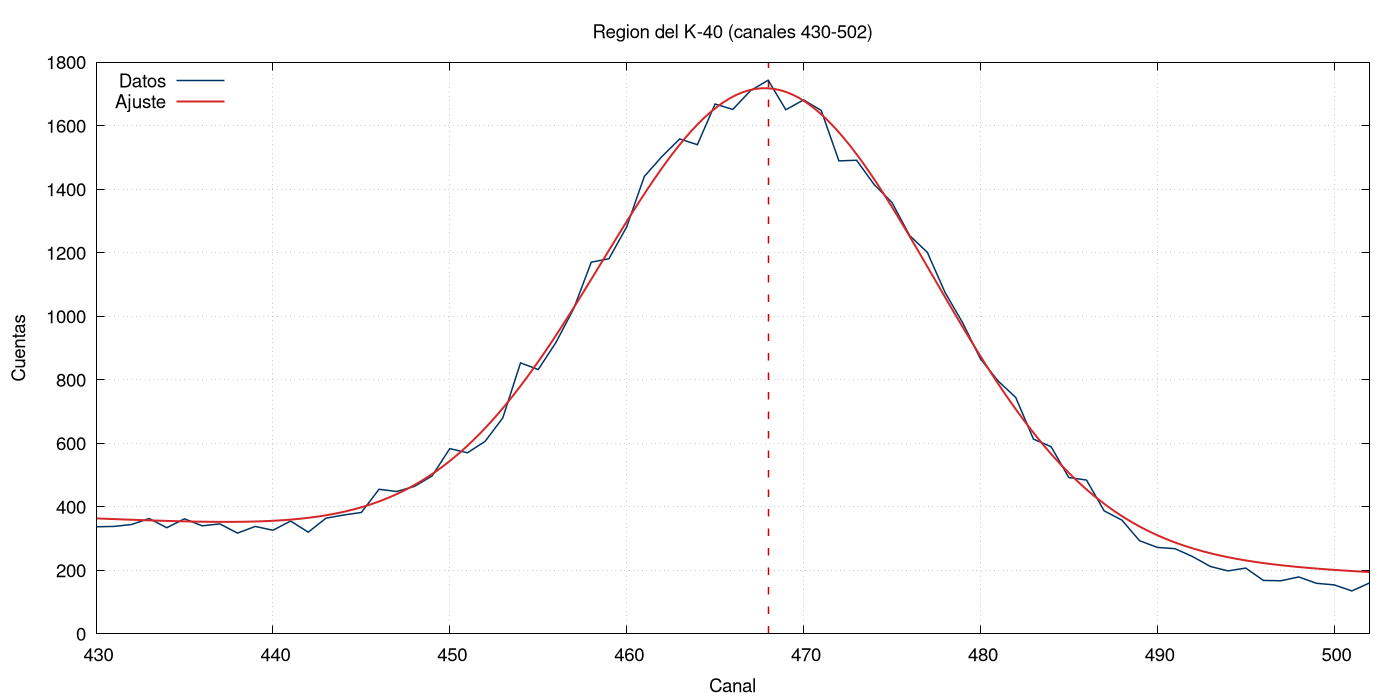
\includegraphics[width=\textwidth]{plots/nal_k40_region.png}
\caption{Zoom a la regi\'on del $^{40}$K (canales 430--502). L\'inea roja: centroide del ajuste.}
\label{fig:nal_k40_region}
\end{figure}

\subsection{Discusi\'on}

La tasa neta de $^{40}$K en el NaI(Tl) (5.31~cps) es mayor que en el REGe (0.305~cps) debido
al mayor volumen y eficiencia del detector NaI. Sin embargo, la resoluci\'on es mucho peor
(FWHM~69~keV en NaI vs 1.56~keV en el HPGe), lo que impide resolver picos cercanos.

El $\chi^2$ reducido del ajuste para el $^{40}$K es $\chi^2_{\nu}=3.0$, aceptable para
detectores de centelleo NaI(Tl) cuyos picos no son perfectamente gaussianos y cuyo fondo
no es estrictamente lineal en intervalos amplios. Para el pico de aniquilaci\'on, que es
solo un hombro en el continuo de Compton, el $\chi^2_{\nu}=19.6$ refleja las mayores
desviaciones del modelo gaussiano ideal en esa regi\'on.

\end{document}
